\section{Static Resource Allocation Experiments}\label{eval-static}

%V.	Evaluation
%	a.	Models
%		i.	Model Accuracy
%			1.	Matlab
%		ii.	Performance/Overhead
%			1.	Tess
%				a.	Time to build the model
%				b.	Phase Change Reaction
%		i.	Video Application adding threads
%		ii.	Time to react to phase changes
%		iii.	Show model accuracy through transition?
%	b.	Decisions
%		i.	Decision Accuracy
%			1.	Matlab
%		ii.	Performance/Overhead
%			1.	Tess

We use two different implementations of the \pacora framework for evaluation. Our static framework, described in this Section, collects data online using an x86 processor running Linux and uses that data to build models and make static resource allocation decisions.  Our dynamic framework implemented in a research-prototype manycore operating system, \tess, is presented in Section~\ref{eval-dynamic}.

Our static framework was designed to test the effectiveness of \pacora's model-based convex optimization for allocating resources.  We used it to experiment with the accuracy of different types of models and test the quality of the resource allocation decisions. Data is collected online by running application benchmarks on a recent x86 processor running Linux-2.6.36.  The measured data is processed using Python and then fed to MATLAB~\cite{matlab} to build the RTFs.  MATLAB uses the RTFs to make resource allocation decisions.  We compare performance of the chosen resource allocations with the actual measured performance of all possible resource allocations to test quality of the resource allocation decisions. We use CVX~\cite{cvx} in MATLAB to perform the convex optimization for building RTFs and making resource allocation decisions.  We chose this static approach because it let us test many applications, 44 in total, and many resource allocations rapidly.

\subsection{Platform}

To collect data, we use a prototype version of Intel's Sandy Bridge x86 processor that is similar to the
commercially available client chip, but with additional hardware
support for way-based LLC partitioning.
The Sandy Bridge client chip has 4 quad-issue out-of-order
superscalar cores, each of which supports 2 hyperthreads using
simultaneous multithreading~\cite{IntelRefManual:2011}.
%Each core has private \wunits{32}{KB} instruction and data caches, as well as a
%\wunits{256}{KB} private non-inclusive L2 cache.
The LLC is a 12-way
set-associative \wunits{6}{MB} inclusive L3 cache, shared among all
cores using a ring-based interconnect.
%All three cache levels are write-back.
The cache partitioning mechanism is way-based and works by modifying the
cache-replacement algorithm.  To allocate cache ways, we assign a subset of
the 12 ways to a set of hyperthreads, thereby allowing only those hyperthreads to replace data in those ways.

%Way allocations can be completely private,
%completely shared, or overlapping.  Although all cores can hit on data stored in
%any way, a core can only replace data in its assigned
%ways.   Data is not flushed when the way allocation changes.

We use a customized BIOS that enables the cache partitioning
mechanism, and run unmodified Linux-2.6.36 for all of our experiments.
To allocate cores, we use the Linux {\tt taskset} command to pin applications to
sets of hyperthreads. The standard Linux scheduler performs the scheduling for applications within these containers of hyperthreads. For our experiments we consider each hyperthread to be an independent core. To minimize inter-application interference, we first assign both hyperthreads available in one core before moving on to the next core. For example, a 4-core allocation from \pacora represents 4 hyperthreads on 2 cores on the machine.

\subsection{Performance and Energy Measurement}

To measure application performance, we use the \texttt{libpfm}
library~\cite{Eranian:OLS06,Perfmon2}, built on top of the
\texttt{perf\_events} infrastructure in Linux, to
access available performance counters~\cite{Intel:Manual2012}.

To measure on-chip energy, we use the energy counters available on
Sandy Bridge to measure the consumption of  the entire socket and also
the total combined energy of cores, their private caches, and the
LLC. We access these counters using the Running Average Power Limit
(RAPL) interfaces~\cite{Intel:Manual2012}.  %The counters measure power
%at a $1/2^{16}$ second granularity.

%In addition, we use a FitPC external multimeter to measure at the wall socket the power
%consumed by the entire system, at a
%\wunits{1}{second} granularity.
%We correlate the wall power data with the data collected from the hardware energy counters
%using time stamps.  We observed less than one second of delay in these
%measurements consistently across all experiments.  Together, these
%mechanisms allow us to collect accurate energy readings over the
%entire course of an application's execution.

\subsection{Description of Workloads}

Our workload contains a range of applications from three different
popular benchmark suites: SPEC CPU 2006~\cite{SPEC2006},
DaCapo~\cite{dacapo}, and PARSEC~\cite{parsec}. We selected this set of applications to represent a wide variety of possible resource behaviors in order to properly stress \pacora's RTFs. We include some additional applications to broaden the
scope of the study, and some microbenchmarks to exercise certain
system features.

The \textbf{SPEC CPU2006} benchmark suite~\cite{SPEC2006} is a
CPU-intensive, single-threaded benchmark suite, designed to stress a
system's processor, memory subsystem, and compiler.  Using the
similarity analysis performed by Phansalkar \emph{et
al.}~\cite{Phansalkar:ISCA2007}, we subset the suite, selecting 4
integer benchmarks ({\tt astar}, {\tt libquantum}, {\tt mcf}, {\tt omnetpp}) and 4
floating-point benchmarks (cactusADM, calculix, lbm, povray).  Based
on the characterization study by Jaleel~\cite{Jaleel:TR2007}, we also
pick 4 extra floating-point benchmarks that stress the LLC: {\tt GemsFDTD},
{\tt leslie3d}, {\tt soplex} and {\tt sphinx3}.  When multiple input sets are
available, we pick the single \textit{ref} input indicated by~\cite{Phansalkar:ISCA2007}.

We include the \textbf{DaCapo} Java benchmark suite as a
representative of managed-language workloads. We use the latest 2009 release, which consists of a set of open-source, real-world
applications with non-trivial memory loads, and includes both client and
server-side applications.

The \textbf{PARSEC} benchmark suite is intended to be representative
of parallel real-world applications~\cite{parsec}. PARSEC
programs use various parallelization approaches, including data- and
task-parallelization. We use native input sets and the {\tt pthreads} version for all benchmarks, with the exception of
\texttt{freqmine}, which is only available in OpenMP.

We add four \textbf{additional parallel applications} to help ensure
we cover the space of interest: {\tt Browser\_animation} is a
multithreaded kernel representing a browser layout animation; {\tt
  G500\_csr} code is a breadth-first search algorithm; {\tt Paradecoder} is a parallel
speech-recognition application that takes audio waveforms of human
speech and infers the most likely word sequence intended by the
speaker; {\tt Stencilprobe} simulates heat transfer in a fluid
using a parallel stencil kernel over a regular
grid~\cite{Kamil:Stencilprobe}.

We also add two \textbf{microbenchmarks} that stress the memory
system and cause increased interference between applications: {\tt stream\_uncached} is a memory and on-chip bandwidth hog
that continuously brings data from memory without caching it, while
{\tt ccbench} explores arrays of different sizes to determine the
structure of the cache hierarchy.

Using a performance characterization of the applications, we select a subset of the benchmarks that are representative of different possible responses to resource allocations in order to reduce our study to a feasible size.  Similar to \cite{Phansalkar:ISCA2007}, we use machine learning to select representative benchmarks.  We use a
hierarchical clustering algorithm~\cite{Phansalkar:ISCA2007} provided by the Python library \texttt{scipy-cluster} with the \textit{single-linkage} method.  The feature vector contains parameters to represent core scaling, cache scaling, prefetcher sensitivity and bandwidth sensitivity.  The clustering algorithm uses Euclidean distance between vectors to determine clusters.

The clustering results in 6 clusters representing the following (applications at the cluster center are listed in parenthesis):
 \begin{itemize}\itemsep0pt \parskip0pt \parsep5pt
\item no scalability, high cache utility, ({\tt 429.mcf})
\item no scalability, low cache utility, ({\tt 459.gems\-FDTD})
\item high scalability, low cache utility, ({\tt ferret})
\item limited scalability, high cache utility, ({\tt fop})
\item limited scalability, low cache utility, ({\tt dedup})
\item limited scalability, low bandwidth sensitivity, ({\tt batik})
\end{itemize}

%First, we create a feature vector for each application using the values in the previous subsection:
%1) execution time as we increase the number of threads; 2) execution time as we increase the LLC size; 3) prefetcher sensitivity; and 4) bandwidth sensitivity. All metrics are normalized to the interval $[0,1]$. In total we use vectors with 19 features ($7+10+1+1$).

%The clustering algorithm finds the smallest Euclidean distance of a pair of feature vectors and forms a cluster containing that pair. It continues selecting the next smallest distance between a pair and forms another cluster. Linkage criteria can be used to adjust cluster formation. The single-linkage we selected uses the minimum distance between a pair of objects in different clusters to determine the distance between them.

\subsection{RTF Experiments}
\begin{figure*}[!t]
	\begin{center}	
		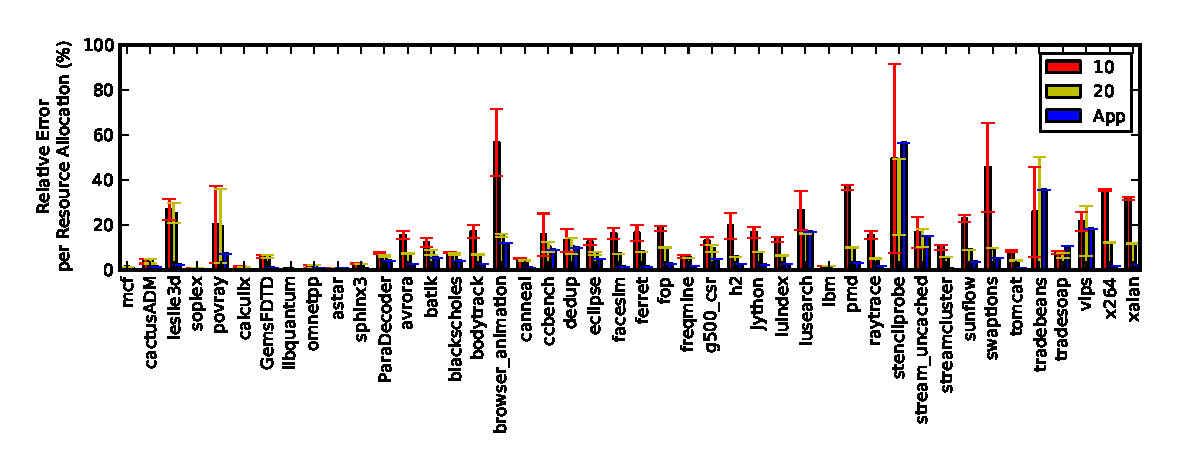
\includegraphics[bb=0 0 576 216,width=\textwidth]{model_accuracy.pdf}
		\caption{1-norm of relative error from RTF predicted response time compared to actual response time.  The actual response time is the median over 3 trials. 10 and 20 represent RTFs built with 10 and 20 training points respectively.  App represents the variability (average standard deviation) in performance of the application between the 3 trials.}
		\label{model_accuracy}
	\end{center}
\end{figure*}
To test the effectiveness of our RTFs in capturing real application behavior, we measure each of our 44 benchmarks running alone on the machine for all possible resource allocations of cache ways and cores.  Cores can be allocated from 1--8 and cache ways from 1--12 resulting in 96 possible allocations for each application.   We use a genetic algorithm design of experiments~\cite{bates-aes03} to select 10 and 20 of the collected allocations to build the RTFs.  We also experimented with building RTFs with more data points but found that they provided little improvement over 20~\cite{pacora_tr}.  We then use the model to predict the performance of every resource allocation and compare it with the actual measured performance (median value of 3 trials) of that resource allocation.  We built 3 different models from 3 trials and tested each of them against median measured value.

Figure~\ref{model_accuracy} shows the 1-norm of the relative error of the predicted response times per resource allocation for an RTF built with 10 training points and one built with 20.  The average error per point is 16\% for an RTF built with 10 training points and 9\% for an RTF built with 20 training points.  We also calculated the percentage variability (average standard deviation) for each resource allocation in the application between the 3 trials (shown as ``App'' in Figure~\ref{model_accuracy}).  The average variability is 9\%, so we can see that \pacora's RTFs are not much more inaccurate than the natural variation in response time in the application.  It is not for possible an RTF to be more accurate than the application variability, and we can also see that applications with higher variability result in RTFs with larger relative errors, (\emph{e.g.,} {\tt stencilprobe}, {\tt tradebeans}).  Section~\ref{discuss} discusses application variability in more detail.


\subsection{Resource Allocation Experiments}
\begin{figure}[!t]
	\begin{center}	
		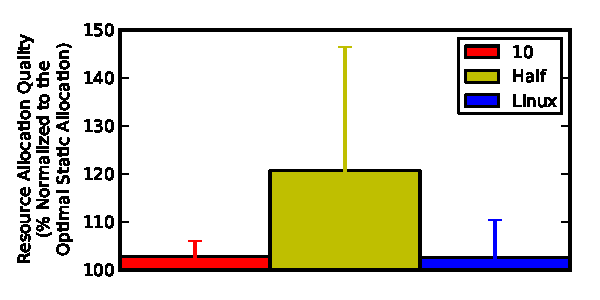
\includegraphics[bb=0 0 288 144,width=\columnwidth]{decision_quality.pdf}
		\caption{Resource allocation decisions for each pair of the cluster representative applications compared equally dividing the machine and a shared resources Linux baseline. Quality is measured is allocation performance divided by performance of the best possible allocation.}
		\label{decision_quality}
	\end{center}
\end{figure}


Using the RTFs built for the applications, we let \pacora make static resource allocations for all possible pairs of the cluster representative applications.  We then run an exhaustive study of all possible resource allocations for each pair on our Sandy Bridge-Linux platform, measure the performance, and compare it with the best performing, \emph{i.e.,} optimal, resource allocation.  We also compare this result to equally dividing the resources between the two applications and to sharing all of the resources using the standard Linux scheduler.

%how \pacora's decisions compared with the optimal allocation, equally dividing the machine, and the Linux baseline for each pair of the cluster representative applications.
Figure~\ref{decision_quality} shows these results for our 10 point RTFs. As we might expect, simple naive heuristics do not perform well, and dividing the machine in half is around 20\% slower than either \pacora or standard Linux.
 \pacora's resource allocations are 2\% from the optimal static allocation on average.  Using shared resources with the standard Linux scheduler performs similarly but with a higher standard deviation.  The shared resources comparison is interesting: while most of the time sharing resources can result in higher utilization, as the applications can dynamically take advantage of available resources, in some cases the interference between applications was so harmful to performance that on average optimal static partitioning performs slightly better.  As a result \pacora is able to provide performance comparable to Linux scheduling on shared resources with more predictable performance on average (lower worst cases).  Additionally, as the shown in the next Section, \pacora's resource allocation decisions do not need to be static, but can be made dynamically to adjust to the changing needs of the applications.


%These results indicate the \pacora is able to get a near optimal resource allocation and match the performance of the traditional Linux scheduler with more predictability.
